\documentclass{article}
\usepackage{graphicx}
\usepackage{amsmath}
\usepackage{amsfonts}
\renewcommand{\baselinestretch}{1}
\setlength{\textheight}{9in}
\setlength{\textwidth}{6.5in}
\setlength{\headheight}{0in}
\setlength{\headsep}{0in}
\setlength{\topmargin}{0in}
\setlength{\oddsidemargin}{0in}
\setlength{\evensidemargin}{0in}
\setlength{\parindent}{.3in}
\graphicspath{{images/}}

\title{Communication Systems \\
    \large Chapter 4 Analog Modulations and Demodulations }
\author{Hunter Mills}
\date{\today}

\begin{document}
    \maketitle

    \medskip
    
    \section{Double-Sideband AM}
    AM is characterized by an information bearing signal $m(t)$ being multiplied by a carrier wave to shift the frequency of the message spectrum to $f_c$.
    \begin{equation}
        m(t) \leftrightarrow M(f)
    \end{equation}
    \begin{equation}
        m(t) \cos 2\pi f_ct \leftrightarrow \frac{1}{2}[M(f+f_c) + M(f-fc)]
    \end{equation}
    Note that the message signal bandwidth at baseband is $B$, but after being modulated by the carrier the AM signal has a bandwidth of $2B$. The portion 
    of the AM bandwidth that is outside of $f_c$ is the \textbf{upper sideband} and the portion inside $f_c$ is the \textbf{lower sideband}. If $M(f)$ does
    not have an impulse at $f=0$ then there will be no discrete component of the carrier $f_c$. In other words the modulation process does not introduce
    a sinusoid at $f_c$. For that reason it is called \textbf{double-sideband suppressed carrier (DSB-SC)}.

    \subsection{Demodulation of DSB-SC}
    I will denote that $\hat{s}(t)$ is the received signal. $\hat{s}(t)$ is first multiplied by a sinusoid of the same frequency and phase as the modulator to 
    move the message, $m(t)$, spectrum back to baseband.
    \begin{equation}
        \hat{s}(t) = m(t) \cos \omega_c t
    \end{equation}
    After multiplication the received signal is 
    \begin{equation}
        \hat{s}(t) = \frac{1}{2}[m(t) + m(t)\cos 2\omega_c t]
    \end{equation}
    This signal is then passed through a low pass filter to get rid of the $m(t)\cos2\omega_ct$ signal that is in the stopband of the filter.

    \subsection{Amplitude Modulators}
    \subsubsection{Nonlinear Modulators}

    \begin{figure}[h]
        \centering
        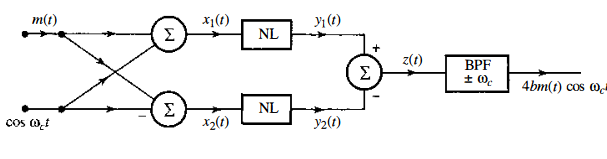
\includegraphics[width=0.75\textwidth]{nl_mod}
        \caption{Nonlinear DSB-SC Modulator}
    \end{figure}

    This block diagram (figure 1) shows a modulator with two identical nonlinear components (marked NL). If the input-output of the nonlinear elements is 
    approximated by the power series:
    \begin{equation}
        y(t) = ax(t) + bx^2(t)
    \end{equation}
    Then
    \begin{equation}
        x(t) = y_1(t) - y_2(t) = [ax_1(t) + bx_1^2(t)] - [ax_2(t) + bx_2^2(t)]
    \end{equation}
    Then subbing $m(t)$ and $\cos\omega_c(t)$ in for $x_1$ and $x_2$ then
    \begin{equation}
        z(t) = 2am(t) + 4bm(t)\cos\omega_ct
    \end{equation}
    Which is then passed through a bandpass filter centered at $f_c$. \\
    \\
    There are multiple more examples of modulators on page 195. 

    \section{Amplitude Modulation}
    In the previous section we talked about DSB-SC because it is easy to walk through. But that simplicity is not good in the real world. Since there is no
    carrier you would need to reproduce a carrier, $\cos[(\omega_c + \Delta\omega)t-\theta_d]$ in the receiver where $\Delta\omega$ is a frequency difference and
    $\theta_d$ is a phase difference. A way to get around that would be to transmit a carrier but the trade off is the transmitter needs to be higher power. 
    This method is conventional \textbf{Amplitude Modulation (AM)}.
    \begin{equation}
        \varphi_{AM}(t) = A\cos\omega_ct + m(t)\cos\omega_ct
    \end{equation}
    \begin{equation}
        \varphi_{AM}(t) = [A + m(t)] \cos\omega_ct
    \end{equation}
    \begin{equation}
        \varphi_{AM}(t) \leftrightarrow \frac{1}{2}[M(f+f_c) + M(f-f_c)] + \frac{A}{2}[\delta(f+f_c) + \delta(f-f_c)]
    \end{equation}
    A condition with AM is that $A$ must be large enough to make $m(t)$ fully positive or it will change the envelope upon demodulation. The \textbf{envelope}
    for the AM signal is defined as 
    \begin{equation}
        |A + m(t)| = A + m(t) \quad \textrm{if the above condition holds}
    \end{equation}

    \begin{figure}[h]
        \centering
        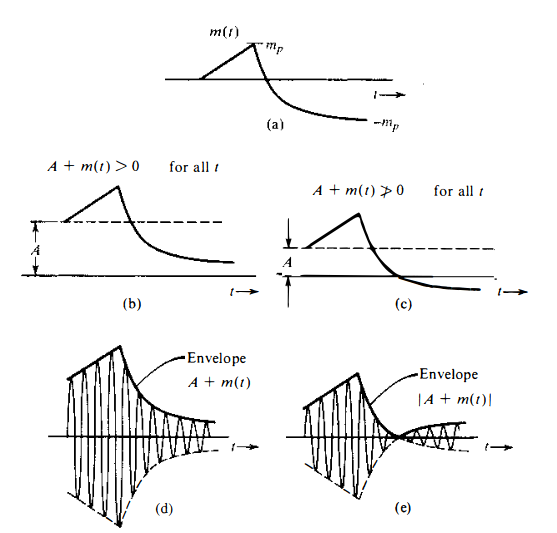
\includegraphics[width=0.75\textwidth]{am_env}
        \caption{Envelope of AM signal}
    \end{figure}

    For envelope detection to work properly $f_c >> m(t)$ bandwidth and $A+m(t) \geq 0$. When a message signal doesnt have any offset, that is
    $-m_{max} = m_{min} = m_p$ (min and max of $m(t)$) are equal then the modulation index is 
    \begin{equation}
        \mu = \frac{m_p}{A} \quad \textrm{where A is the DC offset in the AM signal}
    \end{equation}
    For distortionless envelope detection
    \begin{equation}
        0 \leq \mu \leq 1
    \end{equation}

    When $m_{min} \neq -m_{max}$ then
    \begin{equation}
        \mu = \frac{m_{max}-m_{min}}{2A+m_{max}+m_{min}}
    \end{equation}

    \subsection{Sideband Power, Carrier Power and Modulation Efficiency}
    The advantage of envelope detection in AM is that the carrier carries no information so it can be viewed as wasteful.
    \begin{equation}
        \varphi_{AM}(t) = A\cos \omega_ct + m(t)\cos\omega_ct
    \end{equation}
    The carrier power $P_c$ is the mean square value of $A\cos\omega_ct = A^2/2$. And the sideband power $P_s = <m^2(t)/2>$.

    \subsection{Demodulation of AM Signals}
    You are able to use the same demodulator as in DSB-SC with a PLL for carrier recovery for the mixer. Other ways described in the book (pg 203)
    are with a rectifier and with envelope detection. Figure 2 shows the envelope detector. 

    \begin{figure}[h]
        \centering
        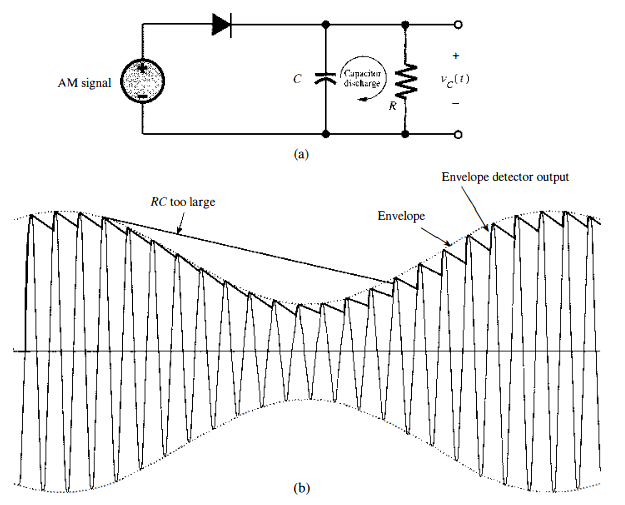
\includegraphics[width=0.75\textwidth]{env_det}
        \caption{Envelope Detector for AM}
    \end{figure}
    where 
    For envelope detection the resistor and capacitor should follow the design criterion of
    \begin{equation}
        \frac{1}{\omega_c} << RC << \frac{1}{2\pi B}
    \end{equation}

    \section{Bandwidth Efficient Amplitude Modulations}
    When transmitting with DSB-SC the message signal $m(t)$ has bandwidth $B$, but the transmitted signal had a bandwidth of $2B$. Two modulation schemes 
    can reduce this phenomenon, \\
    \textbf{1. Single Sideband:} This removes the upper or lower sideband so that the signal only has a transmitted bandwidth of $B$.\\
    \textbf{2. Quadrature AM (QAM):} This utilizes spectral redundancy by sending two messages over the same $2B$.

    \subsection{Single Side Band (SSB)}
    A \textbf{single sideband (SSB)} signal can be demodulated with the same demodulator as the DSB-SC. 

    \subsubsection{Hilbert Transform}
    The \textbf{Hilbert Transform} is defined as 
    \begin{equation}
        x_h(t) = \mathcal{H}{x(t)} = \frac{1}{\pi}\int\frac{x(\alpha)}{t-\alpha}d\alpha
    \end{equation}
    The right hand side has the for of a convolution
    \begin{equation}
        x(t) \ast \frac{1}{\pi t}
    \end{equation}
    Now using the duality property $1/(\pi t) \leftrightarrow -jsgn(f)$ and the application of the convolution property
    \begin{equation}
        X_h(f) = -jX(f)sgn(f) = \begin{cases}
                                    -j=1e^{-j\pi/2} \quad f > 0 \\
                                    j= 1e^{j\pi/2} \quad f < 0
                                \end{cases}
    \end{equation}
    where multiplication with $j$ is a $90$ degree phase shift. Hence the Hilbert Transform is an ideal phase shifter.

    \subsubsection{Time Domain Representation of SSB Signals}
    Let $M_+(f)$ be the upper sideband of the message spectrum and $M_-(f)$ be the lower sideband of the spectrum.
    \begin{equation}
        M_+(f) = M(f)u(f) = M(f)\frac{1}{2}[1 + sgn(f)] = \frac{1}{2}[M(f) + jM_h(f)]
    \end{equation}
    \begin{equation}
        M_-(f) = M(f)u(-f) = M(f)\frac{1}{2}[1 - sgn(f)] = \frac{1}{2}[M(f) - jM_h(f)]
    \end{equation}

    The upper sideband spectrum $\Phi_{USB}(f)$ can be expressed as
    \begin{equation}
        \Phi_{USB}(f) = M_+(f-f_c) + M_-(f+f_c)
    \end{equation}
    \begin{equation}
        \Phi_{USB}(f) = \frac{1}{2}[M(f-f_c)+M(f_c)]-\frac{1}{2j}[H_h(f-f_c) - M_h(f+f_c)]
    \end{equation}
    \begin{equation}
        \varphi_{USB} = m(t) \cos\omega_ct-m_h(t)\sin\omega_ct
    \end{equation}
    \begin{equation}
        \varphi_{SSB} = m(t) \cos\omega_ct \mp m_h(t)\sin\omega_ct
    \end{equation}
    Where the minus sign applies to USB and the plus sign applies to LSB. Figure 3 shows a SSB Modulator with the phase shift method.

    \begin{figure}[h]
        \centering
        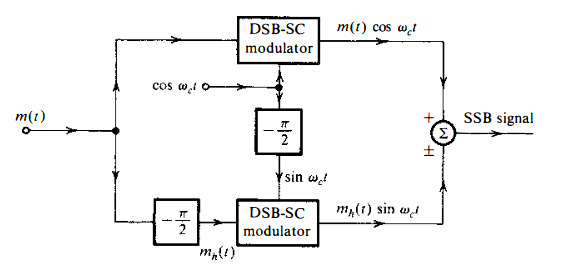
\includegraphics[width=0.75\textwidth]{ssbmod}
        \caption{SSB Modulator}
    \end{figure}

    \subsection{QAM}
    Since SSB modulation is hard to realize in real life \textbf{Quadrature Amplitude Modulation (QAM)} is used. QAM operates by transmitting two DSB signals 
    via the same carrier frequency but in phase quadrature. 

    \begin{figure}[h]
        \centering
        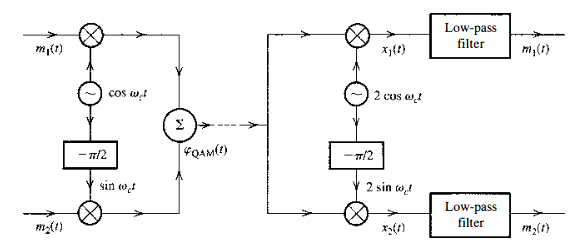
\includegraphics[width=0.75\textwidth]{qam_mod_demod}
        \caption{QAM Modulator and Demodulator}
    \end{figure}

    \begin{equation}
        \varphi_{QAM} (t) = m_1(t)\cos\omega_c t + m_2(t)\sin\omega_ct
    \end{equation}

    In the demodulator
    \begin{equation}
        x_1(t) = 2\varphi_{QAM}(t)\cos\omega_ct = 2[m_1(t)\cos\omega_ct + m_2(t)\sin\omega_ct]\cos\omega_ct
    \end{equation}
    \begin{equation}
        x_1(t) = m_1(t) + m_1(t)\cos\omega_2ct +m_2(t)2\sin\omega_ct
    \end{equation}
    \begin{equation}
        x_2(t) = 2\varphi_{QAM}(t)\sin\omega_ct = 2[m_1(t)\cos\omega_ct + m_2(t)\sin\omega_ct]\sin\omega_ct
    \end{equation}
    \begin{equation}
        x_2(t) = m_2(t) - m_2(t)\cos\omega_2ct +m_1(t)2\sin\omega_ct
    \end{equation}

    QAM demodulations must be totally coherent (frequency and phase). 

    \subsection{Vestigial Sideband (VSB)}
    Since SSB is difficult to generate (Null around DC and an unrealizable phase shifter), another option is \textbf{Vestigial Sideband}. This is a 
    compromise between DSB-SC and SSB. It inherits the advantages of DSB-SC and SSB but avoids their disadvantages at a small price. VSb signals are easy
    to generate and only somewhat higher (about 25-33 percent larger) bandwidth. Unlike SSB were the one half of the spectrum is abruptly cut off,
    the VSB uses a filter to gradually clip the bandwidth. 

    \begin{figure}[h]
        \centering
        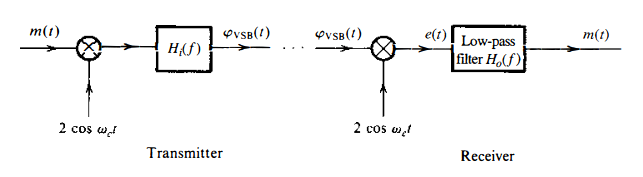
\includegraphics[width=0.75\textwidth]{vsb_mod_demod}
        \caption{VSB Modulator and Demodulator}
    \end{figure}

    \begin{equation}
        \Phi_{VSB}(f) = [M(f+f_c) + M(f-f_c)]H_i(f)
    \end{equation}
    \begin{equation}
        H_o(f) = \frac{1}{H_i(f+f_c) + H_i(f-f_c)} \quad |f| \leq B
    \end{equation}
    where $H_i(f)$ is a bandpass filter. $H_i(f\pm f_c)$ terms contain low pass components.

    \section{Frequency Conversion and Superheterodyne Receivers}
    \subsection{Frequency Mixer of Converter}
    A frequency mixer (converter) can be used to change the carrier frequency of a modulated signal $m(t)$ to another intermediate frequency (IF, $\omega_I$). This 
    can be done by multiplying $m(t)\cos\omega_ct$ by $\cos\omega_{mix}t$ where $\omega_{mix} = \omega_c \pm \omega_I$ before bandpass filtering.

    \begin{equation}
        x(t) = 2m(t)\cos\omega_ct\cos\omega_{mix}t
    \end{equation}
    \begin{equation}
        x(t) = m(t)[\cos(\omega_c -\omega_{mix})t + \cos(\omega_c + \omega_{mix})t]
    \end{equation}

    \subsection{Superheterodyne Receivers}
    A \textbf{Superheterodyne} receiver consists of a RF section, a frequency mixer, and intermediate frequency (IF) amplifier and an envelope detector. 

    \begin{figure}[h]
        \centering
        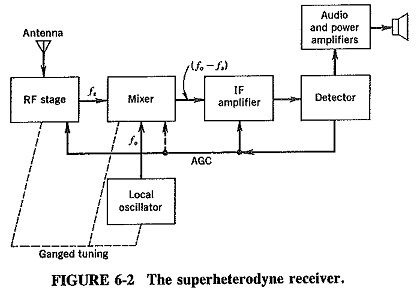
\includegraphics[width=0.75\textwidth]{shr}
        \caption{Superheterodyne Receiver}
    \end{figure}
    where 
    \begin{equation}
        f_{LO} = f_c + f_{IF}
    \end{equation}

    The main reason for the Superheterodyne receiver is for image suppression. Page 238 has good information. 

    \section{Phase Locked Loops}
    A \textbf{PLL} is a device that is used to track the phase and frequency of the carrier component of a signal. It is useful for AM signals with a suppressed
    carrier. A PLL consists of \\
    \textbf{1: } A voltage controlled oscillator (VCO) \\
    \textbf{2: } A multiplier serving as a phase detector or comparator \\
    \textbf{3: } A loop filter $H(s)$.

    \subsection{Basic PLL Operation}
    The VCO is a oscillator whose frequency can be linearly controlled by an input voltage. If the VCO input is $e_o(t)$ then
    \begin{equation}
        \omega(t) = \omega_c + ce_o(t)
    \end{equation}
    where $c$ is a constant of the VCO and $\omega_c$ is the free running angular frequency of the VCO [when $e_o(t) = 0$].

    \begin{figure}[h]
        \centering
        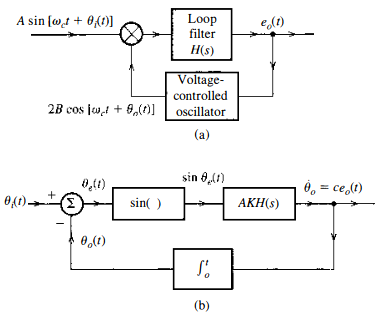
\includegraphics[width=0.75\textwidth]{pll}
        \caption{PLL and its equivalent circuit}
    \end{figure}

    The multiplier output is low pass filtered and then applied to the VCO as an input. The voltage changes the frequency of the oscillator and keeps the loop
    locked by forcing the VCO output to track the phase (and hence the frequency) of the input sinusoid. If the VCO output is $B\cos[\omega_ct + \theta_o(t)]$ 
    then the instantaneous frequency is $\omega_c + \dot{\theta}_o(t)$
    \begin{equation}
        \dot{\theta}_o(t) = ce_o(t)
    \end{equation}
    Let the in coming signal to the PLL be $A\sin[\omega_ct + \theta_i(t)]$, the multiplier output is
    \begin{equation}
        AB\sin(\omega_ct + \theta_i)\cos(\omega_ct + \theta_o) = \frac{AB}{2}[\sin(\theta_i - \theta_0) + \sin(2\omega_ct + \theta_i + \theta_o)]
    \end{equation}
    The second term is suppressed by the loop filter so (where $h(t)$ is the unit impulse response)
    \begin{equation}
        e_o(t) = h(t) \ast \frac{1}{2}AB\sin[\theta_i(t) - \theta_o(t)]
    \end{equation}
    \begin{equation}
        e_o(t) = \frac{1}{2}AB \int_{0}^{t}h(t-x)\sin[\theta_i(x) - \theta_o(x)]dx
    \end{equation}
    Letting $K = .5cB$
    \begin{equation}
        \dot{\theta}_o(t) = AK\int_{0}^{t}h(t-x)\sin\theta_e(x)dx
    \end{equation}
    where $\theta_e(t)$ is the phase error defined as 
    \begin{equation}
        \theta_e(t) = \theta_i(t) - \theta_o(t)
    \end{equation}

    The PLL design requires careful selection of $H(s)$ and the loop gain $AK$. For different tracking widths/frequency different parameters need to be used. 

    \subsection{Small Error PLL}
    In small-error PLL analysis, $sin(\theta_e) \approx \theta_e$ and the block diagram reduces from figure 8 to figure 9. 
    \begin{figure}[h]
        \centering
        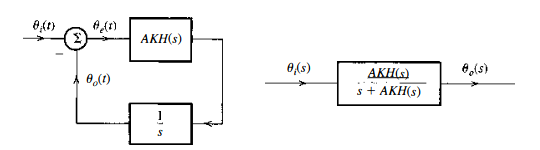
\includegraphics[width=0.75\textwidth]{smallerr}
        \caption{Small Error Linearized PLL}
    \end{figure}

    \begin{equation}
        \frac{\Theta_o(s)}{\Theta_i(s)} = \frac{AKH(s)/s}{1 + {[AKH(s)/s]}} = \frac{AKH(s)}{s+AKH(S)}
    \end{equation}
    The PLL acts as a filter with the above transfer function and the error $\Theta_e(s)$ is given by
    \begin{equation}
        \Theta_e(s) = \frac{s}{s + AKH(s)}\Theta_i(s)
    \end{equation}

    Example on acquisition of frequency when the input signal is $A\sin(\omega_0t + \varphi_0)$. The input signal can be represented as $A\sin[\omega_ct + 
    \theta_i(t)]$ where 
    \begin{equation}
        \theta_i(t) = (\omega_0 - \omega_c)t + \varphi_0
    \end{equation}
    \begin{equation}
        \Theta_i(s) = \frac{\omega_c - \omega_c}{s^2} + \frac{\varphi_0}{s}
    \end{equation}
    When $H(s) = 1$ (first order),
    \begin{equation}
        \Theta_e(s) = \frac{s}{s + AK} [\frac{\omega_c - \omega_c}{s^2} + \frac{\varphi_0}{s}]
    \end{equation}
    \begin{equation}
        \Theta_e(s) = \frac{(\omega_c - \omega_c)/AK}{s} - [\frac{(\omega_c - \omega_c)/AK}{s+AK} + \frac{\varphi_0}{s+AK}]
    \end{equation}
    Hence using the Laplace Transform 
    \begin{equation}
        \theta_e(t) = [\frac{(\omega_c - \omega_c)}{AK}(1-e^{-AKt}) + \varphi_oe^{-AKt}]u(t)
    \end{equation}
    Observe that 
    \begin{equation}
        \lim_{t\rightarrow \infty} \theta_e(t) = \frac{\omega_0 -\omega_c}{AK}
    \end{equation}
    This limit is the constant phase offset when the PLL locks onto the carrier. To get a phase lock:
    \begin{equation}
        \lim_{t\rightarrow \infty} \theta_e(t) = \lim_{s\rightarrow 0} \Theta_e(s) = 0
    \end{equation}
    In which case the loop filter must be greater than first order. 


    \section{FM and PM: Nonlinear Angle Modulations}
    For a general sinusoid
    \begin{equation}
        \varphi(t) = A\cos\theta(t)
    \end{equation}
    where $\theta(t)$ is the generalized angle the instantaneous frequency is
    \begin{equation}
        \omega_i(t) = \frac{d\theta}{dt}
    \end{equation}
    \begin{equation}
        \theta(t) = \int_{-\infty}^{t}\omega_i(\alpha)d\alpha
    \end{equation}
    This shows that you can transmit information $m(t)$ by varying the angle $\theta$ of the carrier. In \textbf{Phase Modulation (PM)} the angle
    $\theta(t)$ is varied linearly with $m(t)$:
    \begin{equation}
        \theta(t) = \omega_ct + k_pm(t)
    \end{equation}
    where $k_p$ is a constant and $\omega_c$ is the carrier. The resulting \textbf{PM} wave is
    \begin{equation}
        \varphi_{PM}(t) = A\cos[\omega_ct + k_pm(t)]
    \end{equation}

    The instantaneous frequency is 
    \begin{equation}
        \omega_i(t) = \frac{d\theta}{dt} = \omega_c + k_p\dot{m}(t)
    \end{equation}
    Hence in PM the instantaneous angular frequency varies linearly with the derivative of $m(t)$. If the instantaneous frequency is valried linearly with
    $m(t)$ then we have \textbf{FM}. 
    \begin{equation}
        \omega_i(t) = \omega_c + k_fm(t)
    \end{equation}
    \begin{equation}
        \theta(t) = \int_{-\infty}^{t}[\omega_c + k_fm(\alpha)]d\alpha
    \end{equation}
    \begin{equation}
        \theta(t) = \omega_ct + k_f\int_{-\infty}^{t}m(\alpha)d\alpha
    \end{equation}
    \begin{equation}
        \varphi_{FM}(t) = A\cos[\omega_ct + k_f\int_{-\infty}^{t}m(\alpha)d\alpha]
    \end{equation}
    FM and PM have a constant power no matter $k_f$ or $k_p$ which is $A^2/2$.

    \begin{figure}[h]
        \centering
        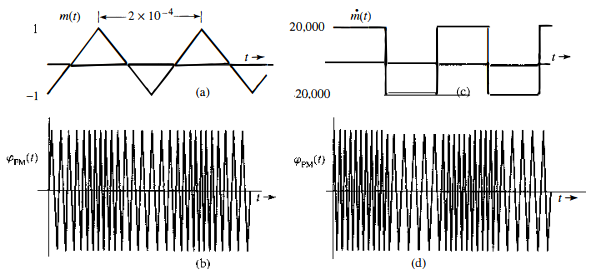
\includegraphics[width=0.75\textwidth]{fm_pm}
        \caption{FM vs PM}
    \end{figure}

    When $m(t)$ is a digital modulation signal, $\dot{m}(t)$ are delta functions at the level changes. This causes instantaneous phase shift called
    phase shift keying. When there are discontinuities in the signal $k_pm(t)$ must stay in the range $[-\pi, \pi]$. 

    \section{Bandwidth Analysis of Angle Modulations}
    There are two types of FM, \textbf{Narrowband FM} and \textbf{Wideband FM}. 

    \begin{equation}
        a(t) = \int_{-\infty}^{t}m(\alpha)d\alpha
    \end{equation}

    \subsection{Narrowband Angle Modulation}
    \textbf{Narrowband FM} is when 
    \begin{equation}
        |k_f|a(t) << 1
    \end{equation}
    Then the approximation 
    \begin{equation}
        \varphi_{FM} \approx A[\cos\omega_ct-k_fa(t)\sin\omega_ct]
    \end{equation}
    Similarly \textbf{narrowband PM} is 
    \begin{equation}
        \varphi_{PM} \approx A[\cos\omega_ct-k_fm(t)\sin\omega_ct]
    \end{equation}
    
    Both have an approximate bandwidth of $2B$.

    \subsection{Wideband FM}
    The peak frequency deviation $\Delta f$ is defined as
    \begin{equation}
        \Delta f = k_f \frac{m_max-m_min}{4\pi}
    \end{equation}
    and the estimated bandwith can be (larger than real bandwidth since derived in book as staircase function)
    \begin{equation}
        B_{FM} = \approx 2(\Delta f + 2B)
    \end{equation}
    where the real bandwidth is in the range $[2\Delta f, 2\Delta f + 4B]$
    A better bandwidth estimate is known as \textbf{Carson's Rule}
    \begin{equation}
        B_{FM} = 2(\Delta f + B) = 2(\frac{k_fm_p}{2\pi} + B)
    \end{equation}
    And for a truly wideband FM signal 
    \begin{equation}
        B_{FM} \approx 2\Delta f \quad \delta f >> B
    \end{equation}

    The deviation ratio $\beta$ is
    \begin{equation}
        \beta = \frac{\Delta f}{B}
    \end{equation}
    Where Carson's rule for estimating FM bandwidth is 
    \begin{equation}
        B_{FM} = 2B(\beta + 1)
    \end{equation}

    \subsection{Phase Modulation}
    \begin{equation}
        \Delta f = k_p \frac{[\dot{m}(t)]_{max} - [\dot{m}(t)]_{min}}{4\pi}
    \end{equation}
    \begin{equation}
        \beta = \frac{\Delta f}{B}
    \end{equation}

    \begin{equation}
        \Delta f = k_p \frac{\dot{m}(t)}{2\pi}
    \end{equation}
    Therefor the PM bandwidth is approximately 
    \begin{equation}
        B_{PM} = 2(\Delta f + B)
    \end{equation}
    \begin{equation}
        B_{PM} = 2B(\beta + 1)
    \end{equation}

    For FM $\Delta f$ only depends on the peak of $m(t)$ and is independent of the spectrum $M(f)$. PM on the other hand depends on the peak of 
    $\dot{m}(t)$ which depends on the spectrum $M(f)$. So the FM bandwidth is practically independent of the spectral shape of $m(t)$ where the PM 
    bandwidth is strongly affected by it.

    \section{Demodulation of FM Signals}
    The information in FM is in the instantaneous frequency so a frequency selective network with a transfer function of $|H(f)| = 2a\pi f + b$
    over the FM band would yield an output proportion to the instantaneous frequency. One type is an ideal differentiator with $|H(f)| = j2\pi f$.
    If we apply $\varphi_{FM}(t)$ to this transfer function
    \begin{equation}
        \dot{\varphi}_{FM}(t) = \frac{d}{dt}{A\cos[\omega_ct +k_f\int_{-\infty}^{t}m(\alpha)d\alpha]}
    \end{equation}
    \begin{equation}
        \dot{\varphi}_{FM}(t) = A[\omega_c + k_fm(t)]\sin[\omega_ct +k_f\int_{-\infty}^{t}m(\alpha)d\alpha - \pi]
    \end{equation}
    and $m(t)$ can be recovered with an envelope detector. 

    \begin{figure}[h]
        \centering
        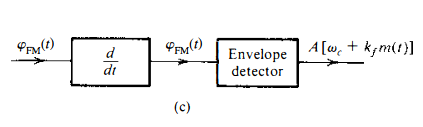
\includegraphics[width=0.75\textwidth]{fm_demod}
        \caption{FM Demodulator}
    \end{figure}

\end{document}